\documentclass{beamer}

\usepackage{txfonts}
\usepackage{hyperref}
\usepackage{fancybox}
\usepackage{xfrac}
\usepackage{cancel}

\newcommand{\heart}{\ensuremath\heartsuit}

\usepackage{mathtools,amssymb}
\newcommand{\myarrow}{\scalebox{2}[2]{$\mathclap{\curvearrowleft}\mkern2.2mu
                                                 \mathclap{\curvearrowright}$}}

\DeclareMathOperator{\Bin}{\mathrm{Bin}}

\hypersetup{colorlinks=false,linkbordercolor=red,linkcolor=green,pdfborderstyle={/S/U/W 1}}

\addtobeamertemplate{navigation symbols}{}{ \hspace{1em}    \usebeamerfont{footline}%
    \insertframenumber / \inserttotalframenumber}

\geometry{papersize={15cm,15cm}}
\usepackage{lipsum}

\makeatletter
\newenvironment<>{contdproof}[1][\proofname]{%
    \par
    \def\insertproofname{#1\@addpunct{.}}%
    \usebeamertemplate{proof begin}#2}
  {\usebeamertemplate{proof end}}
\makeatother


\setbeamertemplate{theorems}[numbered]

\newtheorem*{nonumdefinition}{Definition}
\newtheorem*{nonumproblem}{Problem}
\newtheorem*{nonumproof}{Proof}
\newtheorem*{nonumtheorem}{Theorem}
\newtheorem*{nonumremark}{Remark}
\newtheorem*{answer}{Answer}
\newtheorem*{nonumremarks}{Remarks}
\newtheorem*{nonumexamples}{Examples}
\newtheorem*{nonumsolution}{Solution}
\newtheorem*{nonumexample}{Example}
\newtheorem*{nonumproposition}{Proposition}
\newtheorem{proposition}[theorem]{Proposition}

\usepackage{tikz}
\newcommand*\mycirc[1]{%
  \tikz[baseline=(C.base)]\node[draw,circle,inner sep=.7pt](C) {#1};\:
}

\newcommand\myheading[1]{%
  \par\bigskip
  {\color{blue}{\large #1}}\par\smallskip}

%\usetheme{Warsaw}
%\usetheme{Berkeley} %sample 1

\usetheme{Berlin} % sample 2
%\usetheme{AnnArbor} % sample 3

\let\otp\titlepage
\renewcommand{\titlepage}{\otp\addtocounter{framenumber}{-1}}

\title{Lecture 12 : The Basic Continuous Distributions}
\author{}
\date{}

\begin{document}
\begin{frame}[plain]
\titlepage
\end{frame}

\begin{frame}
We will now study the basic examples

\medskip
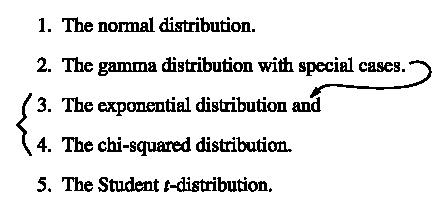
\includegraphics[scale=1.2]{figure/fig1.eps}

\medskip

\underline{This is the most important lecture in the course.}
\end{frame}

\begin{frame}
This lecture is all about the most important distribution.

\myheading{The Normal Distribution}

\begin{nonumdefinition}
A continuous random variable $X$ has normal distribution with parameters $\mu$ and $\sigma^{2}$, denoted $X\sim N(\mu, \sigma^{2})$, if the pdf $f$ of $X$ is given by
$$
f(x)=\dfrac{1}{\sqrt{2\pi}\sigma} e^{-\frac{1}{2}\left(\frac{X-\mu}{\sigma}\right)^{2}}, \ -\infty<x<-\infty
$$
The graph of $f$ is the ``bell curve''

\medskip
\centerline{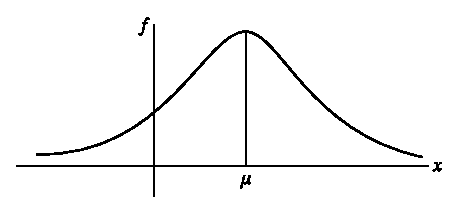
\includegraphics{figure/fig2.eps}}
\end{nonumdefinition}
\end{frame}

\begin{frame}
\begin{nonumdefinition}[Cont.]
$\mu$ is a point of symmetry of $f$ so by Lecture 11, page 15
$$
E(X)=\mu.
$$
(this why this parameter is called $\mu$).

$\sigma^{2}$ measures The ``width'' of the curve

\medskip
\centerline{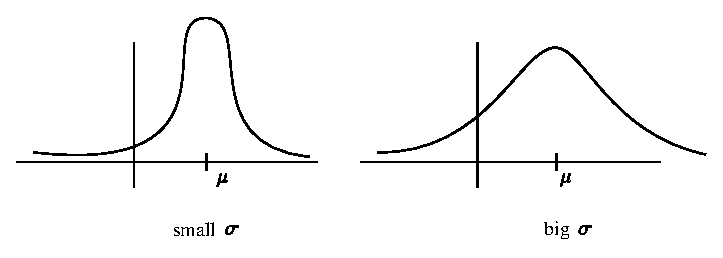
\includegraphics{figure/fig3.eps}}
\end{nonumdefinition}

\begin{nonumproposition}
If $X\sim N(\mu, \sigma^{2})$ then
\begin{itemize}
\item[(i)] $E(X)=\mu$

\item[(ii)] $V(X)=\sigma^{2}$
\end{itemize}
(this justifies the names of the parameters)
\end{nonumproposition}
\end{frame}

\begin{frame}
\begin{nonumremark}
If $X\sim N(\mu,\sigma^{2})$ then
$$
P(a\leq X\leq b)=\int\limits^{b}_{a}\frac{1}{\sqrt{2\pi}\sigma}e^{-\frac{1}{2}(\frac{X-\mu}{\sigma})^{2}}dx
$$
This integral cannot be computed by calculus methods so it must be computed by numerical analysis methods. However these probabilities can be recovered from the table in the front flip text or from a computer. To do this we need to reduce to the ``standard'' case $\mu=0$, $\sigma=1$ (otherwise we would need infinitely many tables, one for each pair $(\mu,\sigma^{2})$). The reduction to the standard case is called \underline{standardization}.
\end{nonumremark}
\end{frame}

\begin{frame}
\myheading{The Standard Normal Distribution}

\begin{nonumdefinition}
A normal distribution with mean $0$ and variance $1$ (so $\mu=0$ and $\sigma^{2}=1$, so $\sigma=1$) is called a \underline{standard normal distribution}.

A random variable with standard normal distribution will be denoted $Z$ so $Z\sim N(0,1)$.

The pdf $f(z)$ for $Z$ is given by
$$
f(z)=\dfrac{1}{\sqrt{2\pi}} e^{-\frac{1}{2}z^{2}}, -\infty < z<-\infty
$$
(see the next page for the graph of $f$)

The function on the right is often called the Gaussian and comes up all over mathematics. It gives rise to the famous theta functions in number theory.
\end{nonumdefinition}
\end{frame}

\begin{frame}
\begin{nonumdefinition}
The cumulative distribution function of the normal distribution will be denoted $\Phi(z)$. So
$$
\Phi(z)=P(Z\leq z)=\int\limits^{z}_{-\infty}\frac{1}{\sqrt{2\pi}}e^{-\frac{1}{2}t^{2}}dt
$$
\end{nonumdefinition}

\myheading{Pictures}

\centerline{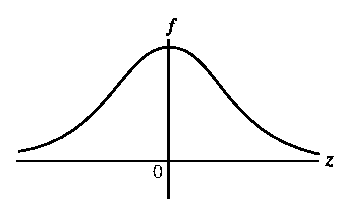
\includegraphics[scale=.85]{figure/fig4.eps}}

\centerline{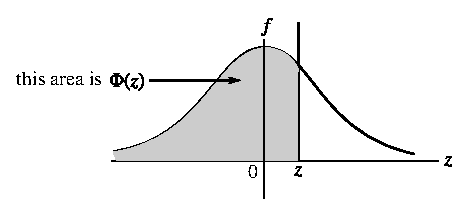
\includegraphics[scale=.9]{figure/fig5.eps}}

\centerline{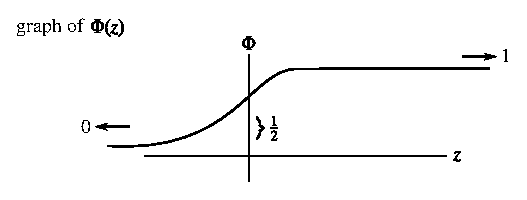
\includegraphics[scale=.9]{figure/fig6.eps}}
\end{frame}

\begin{frame}
$\lim\limits_{z\to -\infty}\Phi(z)=0$

$\lim\limits_{z\to \infty}\Phi(z)=1$

\myheading{Using the tables on page 668-669}

The values of $\Phi(z)$ are tabulated in the front flops of the text or better from the web - see next page.

From the table in the front flop on the web

\begin{nonumproblem}
\begin{itemize}
\item[(a)] Compute $P(Z\leq 1.25) (0.8944)$

\item[(b)] Compute $P(Z\leq -1.25)$

\item[(c)] Compute $P(-1.25\leq Z\leq 1.25)$
\end{itemize}
The challenge is to use the answer to (a) namely $.8944$ to do (b) and (c). In other words to do all three parts you have to look up \underline{only one value}.

First we show (a) gives (b).
\end{nonumproblem}
\end{frame}

\begin{frame}
\centerline{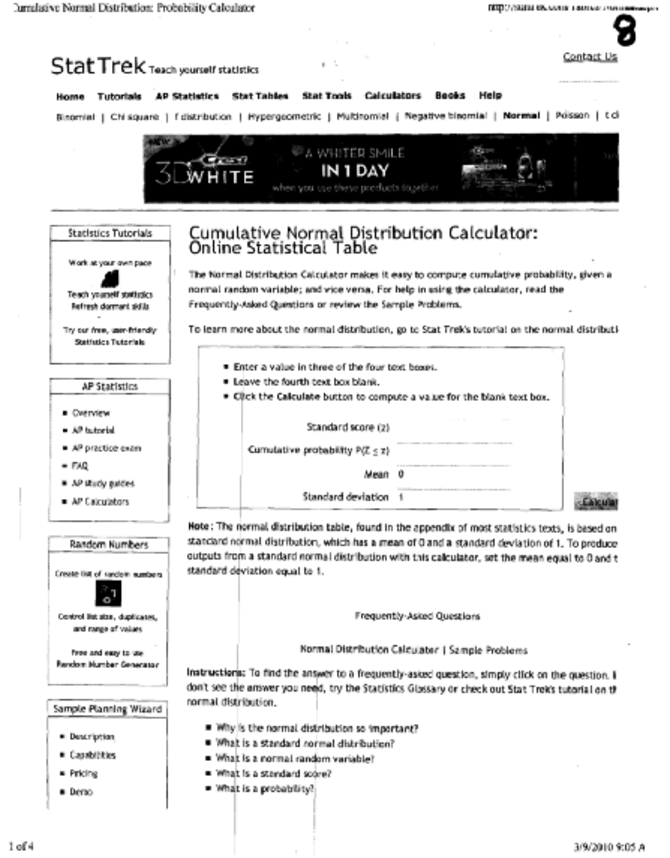
\includegraphics[scale=.9]{figure/fig7.pdf}}
\end{frame}

\begin{frame}
\begin{nonumproblem}[Cont.]
The point is that because $f(z)=\dfrac{1}{2\pi}e^{-\frac{1}{2}z^{2}}$ is even ($f(-z)=f(z)$ because it is a function of $z^{2}$) the function $\Phi(z)$ also has (a more subtle) symmetry namely
\begin{equation*}
\Phi(-a)=1-\Phi(a)\tag{*}
\end{equation*}
It is easiest to state and prove this in terms of probabilities.
\end{nonumproblem}

\begin{nonumproposition}
\begin{equation*}
P(Z\leq -a)=1-P(Z\leq a)\tag{**}
\end{equation*}
(*) and (**) are the same
\end{nonumproposition}
\end{frame}

\begin{frame}
\begin{proof}
\centerline{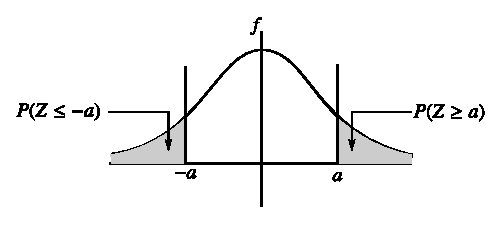
\includegraphics{figure/fig8.eps}}
\smallskip

Because $f(z)$ is symmetric about the $y$ axis $(f(-z)=f(z))$ the two shaded areas have to be the same. Since one is the mirror image of other (where the $y$-axis is the mirror). Hence
$$
P(Z\leq -a)=P(Z\geq a)=1-P(Z<a)
$$
(because $(Z\geq a)$ and $(Z<a)$ are complements of each other).

But $Z$ is continuous so
$$
P(Z<a)=P(Z\leq a)\quad\text{and}\quad P(Z\leq -a)=1-P(Z\leq a)
$$
\end{proof}
\end{frame}

\begin{frame}
Now we can do (b) given the answer to (a)
\begin{align*}
P(Z\leq -1.25) &=1-P(Z\leq 1.25)\\
               &=1-.8944\\
               &=.1056
\end{align*}
Now what about (c). We have 
$$
P(-a\leq Z\leq a)=2\Phi(a)=1
$$
\begin{proof}
\centerline{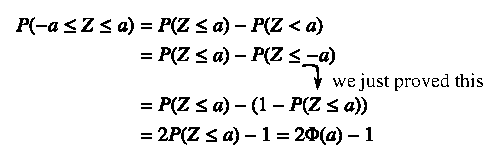
\includegraphics{figure/fig9.eps}}
\end{proof}
\end{frame}

\begin{frame}
So now we can do (c) using (a)
\begin{align*}
& P(-1.25\leq Z\leq 1.25)=2\Phi(1.25)-1\\
&\quad =2(.8944)-1=.7888
\end{align*}
So we repeat - \underline{all we needed to do all three parts was the one value}
$$
\Phi(1.25)=P(Z\leq 1.25)=.8944
$$

\myheading{The $\alpha$-th critical value $z_{\alpha}$ of the standard normal}

Let $\alpha$ be a real numbers between $0$ and $1$. We review the definition of the $\alpha$-th critical value $z_{\alpha}$ (we have change $X$ to $Z$) from Lecture 11, pages 5, 6, 7.
\end{frame}

\begin{frame}
$z_{\alpha}$ is the number so that the vertical line $z=z_{\alpha}$ cuts off area $\alpha$ to the \underline{right} under the graph of $f(z)=\dfrac{1}{\sqrt{2\pi}}e^{-\frac{z^{2}}{2}}$.

\smallskip
\centerline{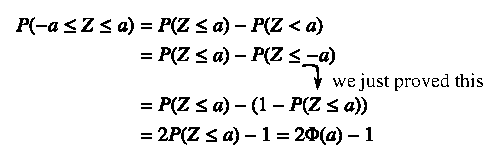
\includegraphics{figure/fig9.eps}}
\smallskip

Equivalently,
\begin{align*}
P(Z\geq z_{\alpha}) &= \alpha\\
\text{or}\quad 1-P(Z\leq z_{\alpha}) &=\alpha\\
P(Z\leq z_{\alpha}) &= 1-\alpha\\
\Phi(z_{\alpha}) &=1-\alpha\\
z_{\alpha} &= \Phi^{-1}(1-\alpha)
\end{align*}
\end{frame}

\begin{frame}
The values of $z_{\alpha}$ may be obtained from page 148 of the text or better, the bark flap of the text, Table A.S.

\smallskip
\centerline{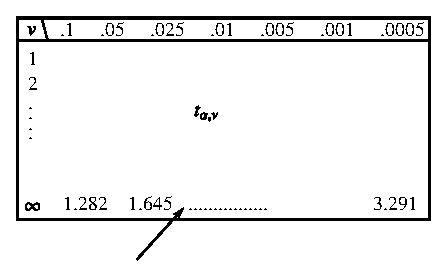
\includegraphics{figure/fig11.eps}}
\smallskip

It may not look like it but the bottom now gives the values of $z_{\alpha}$ for 
$$
\alpha=.1, \ .05, \ .025, \ .01, \ .005, \ .001, \ .0005
$$
This is because
$$
\lim\limits_{v\to \infty}t_{\alpha,\nu}=z_{\alpha}
$$
\end{frame}

\begin{frame}
It will be important if you go further in statistics to think of $z_{\alpha}$ as a function of $\alpha$, $z_{\alpha}=f(\alpha)$.

What is the graph of $f$?

Here is the answer

\smallskip
\centerline{
\includegraphics{figure/fig12.eps}}
\smallskip

\myheading{Hard Problem}

Prove this using operations on graphs and the formula $z_{\alpha}=\Phi^{-1}(1-\alpha)$
\begin{enumerate}
\item Start with the graph of $\Phi(z)$

\smallskip
\centerline{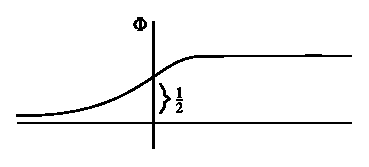
\includegraphics{figure/fig13.eps}}
\smallskip

\item Draw the graph of $\Phi^{-1}(z)$ then of $\Phi^{-1}(1-z)$ (you do this by ``flopping'' graphs).
\end{enumerate}
\end{frame}

\begin{frame}
\myheading{Standardizing Everybody has to learn how to do this!}

When $X\sim N(\mu,\sigma^{2})$ the probabilities $P(a\leq X\leq b)$ are computed by ``standardizing'' $X$. The procedure is based on

\begin{nonumproposition}
If $X\sim N(\mu,\sigma^{2})$ then the new random variable $Z=\dfrac{X-\mu}{\sigma}$ satisfies $Z\sim N(0,1)$.
\end{nonumproposition}
\end{frame}

\begin{frame}
\begin{nonumremark}
{\large\bf Z} This may be too hard.

This is a linear change of continuous random variable. We haven't defined change of continuous random variable but we will say something how.
\end{nonumremark}

\myheading{Here is the idea}

Write the density of $X$ as 
$$
f(x)dx=\dfrac{1}{\sqrt{2\pi \sigma}}e^{-\frac{1}{2}\left(\frac{X-\mu}{\sigma}\right)^{2}}dx
$$
\underline{you have to put in the $dx$ here.}

\smallskip

Now substitute $Z=\dfrac{X-\mu}{\sigma}$ on $X=\sigma 2+\mu$ so $dx=\sigma dz$ so when we e-express the right-hand side in terms of $z$ we get

\medskip
\centerline{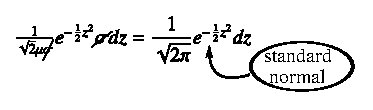
\includegraphics{figure/fig14.eps}}
\end{frame}

\begin{frame}
In general when you make a change of variance from $X$ to $Y=h(X)$ you take the density $F(x)dx$ of $X$ and re-express everything in terms of $y$ using $X=h^{-1}(y)$ so $dx=d(h^{-1}(g))$. 

This is the idea but need tightening up.

\myheading{Now back to Stat 400 and what you absolutely have to know}

\begin{nonumexample}
Suppose \ $X\sim N(40,(1.5)^{2})$

Compute \ $P(39\leq X\leq 42)$
\end{nonumexample}
\end{frame}

\begin{frame}
\begin{nonumsolution}
Be careful : $\sigma^{2}=(1.5)^{2}$ so $\sigma=1.5$, you have to divide by $\sigma=1.5$ below.

The desired probability is $P(39\leq X\leq 42)$

We subtract the mean $\mu=40$ from EVERYTHING and divide EVERYTHING by $\sigma=1.5$. This way we have an equality

\smallskip
\centerline{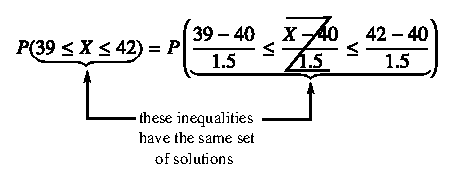
\includegraphics{figure/fig15.eps}}
\smallskip

because we have done the some thing to all terms in the inequalities on the left.
\end{nonumsolution}
\end{frame}

\begin{frame}
\begin{nonumsolution}[Cont.]
We obtain
\begin{align*}
& P(39\leq X\leq 42)=P\left(-\dfrac{1}{1.5}\leq Z\leq \dfrac{-2}{1.5}\right)\\
&\quad =P\left(-\dfrac{2}{3}\leq Z\leq \dfrac{4}{3}\right)\\
&\quad =P(-.67\leq Z\leq 1.33)\\
&\quad =\Phi(1.33)-\Phi(-.67)\\
&\text{from front flop}\\
&\quad =.9082-.2514\\
&\quad =.6568
\end{align*}
\end{nonumsolution}
\underline{Make sure you understand this computation completely.}
\end{frame}

\begin{frame}
In real-life problems you might not have a table available. Still you can give a good approximation to normal probabilities using the

\myheading{Two-Sided Rule of Thumb, page 151}


Let $X\sim N(\mu,\sigma^{2})$. We will give approximations for $X$ to be within 1, 2 and 3 standard deviations of its mean

\myheading{(1) One standard deviation}
$$
P(|X-\mu|\leq \sigma)\approx .68 
$$
\end{frame}

\begin{frame}
\smallskip
\centerline{\includegraphics{figure/fig16.eps}}
\smallskip

\myheading{(2) Two standard deviations}
\smallskip
\centerline{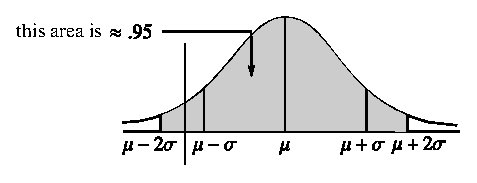
\includegraphics{figure/fig17.eps}}
$$
P(|X-\mu|\leq 2\sigma)\approx .95
$$

\myheading{(3) Three standard deviations}

\smallskip
\centerline{\includegraphics{figure/fig18.eps}}
$$
P(|X-\mu|\leq 3\sigma)\approx .997
$$
\end{frame}

\begin{frame}
Consequence (we will need these)

\myheading{The One-Sided Rule of Thumb One standard deviation}
$$
P(X-\mu>\sigma)\approx .16
$$
\smallskip
\centerline{\includegraphics{figure/fig19.eps}}

Why

\smallskip
\centerline{\includegraphics{figure/fig21.eps}}
\end{frame}

\begin{frame}
\myheading{Two standard deviations}
$$
P(X-\mu>2\sigma)\approx .025
$$
\centerline{\includegraphics{figure/fig20.eps}}
\smallskip

Left to you.
\end{frame}

\begin{frame}
\myheading{The Normal Approximation to the Binomial}

Recall
\begin{align*}
X\sim \Bin (n,p)\Rightarrow E(X) &= np\\
\text{and}\quad V(X) &= npq
\end{align*}

\begin{nonumtheorem}[Normal approximation to the binomial]
If $X\sim \Bin (n,p)$ and $n$ is large (relative to $p$ and $q$) specifically $np\geq 10$ and $nq\geq 10$ then $X$ is approximately normal. ?????? if $Y$ is the normal random variable with the same mean and variance as $X$.
\end{nonumtheorem}
\end{frame}

\begin{frame}
so $Y\sim (np, npq)$ then for all $a$, $b$.
$$
P(a\leq X\leq b)\approx P(a\leq Y\leq b)
$$

\begin{nonumproblem}
Professional mathematicians would not accept this theorem. \underline{There is no estimate on the error of the approximation.}

On the cosmic scale $1\approx 2$ but not in real life so ``approximate'' is too vague. But in fact the above approximation is good to a large number if decimal places and there is a (complicated) estimate for the error.
\end{nonumproblem}
\end{frame}

\begin{frame}
\myheading{Refinement (not that important) ``Correction for Continuity''}
\begin{equation*}
P(a\leq X\leq b)\approx P(a\leq Y\leq b)\tag{b}\label{eq-b}
\end{equation*}
But $X$ is discrete and $Y$ is continuous so $X$ could assign a non-zero probability to the end $a$ and to the other end $b$ ?????? $X$ \underline{would assign zero probability to each end.}

For example

\smallskip
\centerline{\includegraphics{figure/fig22.eps}}
\end{frame}

\begin{frame}
So the right-hand side is \underline{too small} so we make it bigger by pushing a $\dfrac{1}{2}$ unit to the left and pushing $b$ $\dfrac{1}{2}$ unit to the right. See the text, pg. 153, - have
$$
P(\underbrace{10\leq X\leq 10}_{X=10})\approx P(9.5\leq Y\leq 10.5)
$$

\myheading{Bottom Line}
\begin{equation*}
P(a\leq X\leq b)\approx P\left(a-\frac{1}{2}\leq Y\leq b+\frac{1}{2}\right)\tag{bb}
\end{equation*}
is better than \eqref{eq-b}.
\end{frame}

\begin{frame}
\myheading{The GRE Problem}

(from Tim Darling, foll 1999)

The following problem was on the Graduate Records Exam in mathematics. As you will see it was pretty hard. 

Suppose a fair die is tossed 360 times. The probability a 6 comes up 70 or more times is
\begin{itemize}
\item[(A)] $>.5$

\item[(B)] Between $(.16,.5)$

\item[(C)] Between $(.02,.16)$

\item[(D)] Between $(.01,.02)$

\item[(E)] $<.01$
\end{itemize}
\end{frame}

\begin{frame}
\begin{nonumsolution}
Let $X=\sharp$ of sixes in 360 tosses

\begin{tabbing}
So success \== 6 appears\\[5pt]
\phantom{So~~ } failure  \>= non 6 appears
\end{tabbing}

So
$$
X\sim \Bin \left(360,\frac{1}{6}\right)
$$
and the exact answer is
$$
P(X\geq 70)\text{~ with~ } X\sim \Bin \left(360,\frac{1}{6}\right)
$$
But we need to choose between (A), (B), (C), (D) and (E).

So we need a \underline{number} - If you had a laptop when you took the exam you wouldn't need what comes next.
\end{nonumsolution}
\end{frame}

\begin{frame}
\begin{nonumsolution}[Cont.]
So we use the \underline{normal approximation to $X$}. We have 
\begin{align*}
E(X)=np=(360)\left(\dfrac{1}{6}\right) &=60\\
V(X)=npq=(np)q &= (60)\left(\frac{5}{6}\right)\\
               &= 50
\end{align*}
So let $Y\sim N(60,50)$

\smallskip
\centerline{
\includegraphics{figure/fig23.eps}}
\smallskip

So
\begin{equation*}
P(X\geq 70)\approx P(Y\geq 70)\tag{*}\label{add-eq*}
\end{equation*}
(we don't use the correction for continuity)

But we aren't done yet unless you have a table of normal probabilities with you.
\end{nonumsolution}
\end{frame}

\begin{frame}
\begin{nonumsolution}[Cont.]
So we need the \underline{one-sided rule of thumb.}

We have to compare the right-hand side of \eqref{add-eq*} to 
\begin{align*}
& P(Y-\mu\geq \sigma)\approx .16\quad\text{and}\\
& P(Y-\mu\geq 2\sigma)\approx .025
\end{align*}
Now $\mu=60$ so
$$
P(Y\geq 70)=P(Y-60\geq 10)
$$
So we get lucky, \underline{10 is between $\sigma=7.7$ and $2\sigma=154$}

So

\smallskip
\centerline{\includegraphics{figure/fig24.eps}}
\smallskip

So 
$$
.16 > P(Y-60>10)>.025
$$
\underline{So the answer is (C)}
\end{nonumsolution}
\end{frame}
\end{document}


